% Translator:
% Tianfan Fu: 12.1~12. 3
% Shenjian Zhao: 12.4~12.5
\chapter{应用}
\label{chap:applications}

在本章中,我们介绍了如何使用\gls{DL}来解决\gls{CV},\gls{SR},\gls{NLP}以及其它商业领域中的应用。
首先我们讨论了在大多数\gls{AI}应用中大规模\gls{NN}的实现。
接着,我们介绍了\gls{DL}已经成功应用的几个特定的领域。
尽管\gls{DL}的一个目标是设计能够处理多种任务的算法,然而截止目前应用\gls{DL}仍然需要一些特定的条件。
比如说,\gls{CV}中的任务对每一个样本都需要大量的输入特征(像素)。
\gls{NLP}中对每一个输入特征都需要对大量的可能值(词汇)建模。
% 431

\section{大规模\glsentrytext{DL}}
\label{sec:large_scale_deep_learning}
% 431 

\gls{DL}的基本思想是建立在连接机制上的:尽管\gls{ML}模型中的单个生物性的神经元或者说是单个特征不是智能的,但是大量的神经元或者特征作用在一起往往能够表现出智能。
我们必须着重强调神经元数量必须很大这个事实。
相比于20世纪80年代,今日的\gls{NN}的精度以及处理任务的复杂度都有了巨大的提升,神经元的数量是一个关键的因素。
正如我们在\ref{sec:increasing_model_sizes}节中看到的一样,在过去的三四十年中,网络的规模是以指数级的速度递增的,尽管如今的\gls{ANN}的规模也仅仅和昆虫的神经系统差不多。

由于大规模\gls{NN}的必要性,所以\gls{DL}需要高性能的硬件设施和软件实现。
% 431

\subsection{快速的CPU实现}
\label{sec:fast_cpu_implementations}

传统做法中,\gls{NN}是用单台机器的CPU来训练的。
在今天,这种做法通常被视为是不可取的。
如今,我们通常使用\glssymbol{GPU}或者许多台机器的CPU连接在一起进行计算。
在使用这种昂贵而又复杂的配置之前,研究者们付出了很大的努力来论证CPU无法承担\gls{NN}所需要的巨大的计算量。
% 432 head


描述如何快速的用CPU实现以及超出了本书的讨论范围,但是我们在这里还是要强调通过设计一些特定的CPU上的操作可以大大加快效率。
举个例子,在2011年,最好的CPU在训练\gls{NN}的时候使用\gls{fixed_point_arithmetic}比\gls{float_point_arithmetic}。
通过调整\gls{fixed_point_arithmetic}的实现方式,\citet{Vanhoucke-et-al-2011}获得了相对于一个很强的\gls{float_point_arithmetic}系统3倍的加速。
各个CPU都有各自不同的特性,所以有时候采用\gls{float_point_arithmetic}来实现会更快。
一条重要的准则就是通过特殊设计的数值运算可以获得巨大的回报。
其它的策略,除了选择\gls{fixed_point_arithmetic}或者\gls{float_point_arithmetic}以外,包括了通过优化数据结构来避免高速缓存缺失,使用向量指令。
除了当模型的规模限制了模型的表现时,\gls{ML}的研究者们一般忽略这些实现的细节。
% 432

\subsection{GPU 实现}
\label{sec:gpu_implementations}

许多现代的\gls{NN}的实现是基于\firstall{GPU}。
\glssymbol{GPU}是一种特殊设计的硬件,设计的原始目的是为了处理图形应用。
它的为视频游戏所设计的特性也可以使\gls{NN}的计算受益。
% 432  

视频游戏要求许多操作能够快速的并行的实现。
环境和角色的模型是通过一系列的3D坐标结点来定位的。
为了将大量的3D坐标转化为2D的显示器上的坐标,显卡必须快速的实现矩阵的乘法或者除法。
之后,显卡必须并行的实现对每个像素的计算来确定每个像素点的颜色。
在这两种情况下,计算是非常简单的,并且不包括CPU通常遇到的复杂的分支运算。
比如说,同一个刚体里的每一个结点都会乘上一个相同的矩阵;也就是说,不需要进行一个if的判断来确定需要乘上哪一个矩阵。
计算过程也是完全相互独立的,因此也能够并行操作。
计算过程还包括了处理大量的缓冲和内存以及描述每一个物体的纹理(颜色)如何渲染的位图信息。
这使得显卡能够拥有并行特性以及很高的内存带宽,同时也付出了一些代价,如相比于传统的CPU更慢的时钟速度以及更弱的处理分支运算的能力。
% p 433


与上面描述的实时的图形算法相比,\gls{NN}算法需要的是相同的硬件特性。
\gls{NN}算法涉及大量的参数,激活值,梯度值通过缓冲区,其中在每一次训练迭代中都要被完全的更新。
对于传统的桌面计算机来说,缓冲区是足够大的,所以内存的带宽成为了主要的瓶颈。
相比于CPU,\glssymbol{GPU}的极高的内存带宽成为了一个显著的优势。
\gls{NN}的训练算法通常并不包含分支运算和复杂的控制指令,所以更适用于在GPU上训练。
由于同一层\gls{NN}往往能够被分为多个独立处理的神经元,所以\gls{NN}能够从GPU的并行特性中受益匪浅。
% 433


\glssymbol{GPU}最初是专门为了图形任务而设计的。
随着时间的推移,\glssymbol{GPU}也变得越发的灵活,能够处理转化结点的坐标或者计算像素颜色的任务。
通过将缓冲区中的像素值作为计算的输出值,\glssymbol{GPU}也可以被用在科学计算中。
\citet{Steinkrau2005}在GPU上实现了一个有两层的全连接的\gls{NN},然后获得了相对于基于CPU的基线方法的三倍的加速。
不久以后,\citet{chellapilla:inria-00112631}也论证了相同的技术可以被用来加速训练\gls{supervised}的\gls{CNN}。
% 433


使用显卡来训练\gls{NN}的热度在\firstall{GP_GPU}的发布以后开始爆炸性增长。
这种\gls{GP_GPU}可以执行任意的代码,而并非渲染任务。
NVIDIA的CUDA编程语言使得我们可以用一种像C一样的语言实现任意的代码。
由于相对简便的编程语言,强大的并行能力以及巨大的内存带宽,\gls{GP_GPU}是我们\gls{NN}训练的理想平台。
在它发布以后不久,这个平台就迅速被\gls{DL}的研究者们接纳了\citep{RainaICML09-small,Ciresan-2010}。




如何在\gls{GP_GPU}上写高效的代码依然是一个难题。
在\glssymbol{GPU}上获得很好表现所需要的技术与CPU上的技术有所不同。
比如说,一个好的基于CPU的代码通常被设计为尽可能从cache中读取更多的信息。
然而在\glssymbol{GPU}中,许多信息并不在cache中,所以往往重复计算某个值会比计算它一边在从内存中读取更快。
\glssymbol{GPU}代码是多线程的,各个线程之间必须协调好。
比如说,如果能够把数据\firstgls{coalesced}起来,那么涉及内存的操作一般会更快。
当几个线程同时需要读/写一个值的时候,像这样的\gls{coalesced}作为一次内存操作出现。
不同的\glssymbol{GPU}采用了不同的\gls{coalesced}读/写数据的方式。
通常来说,如果在$n$个线程中,线程$i$对应的是第$i+j$处的内存,其中j是2的某个幂的乘积。
具体的设定在不同的\glssymbol{GPU}中有所区别。
\glssymbol{GPU}的另一个常见的设定是一个组中的所有线程都同时执行同一指令。
这意味着在\glssymbol{GPU}上分支操作是很困难的。
线程被分为一个个称作\firstgls{warp}的小组。
在一个\gls{warp}中的每一个线程在每一个循环中只执行同一指令,所以当同一个\gls{warp}中的不同线程需要执行不同的指令的时候,需要使用串行而非并行的方式。
% 434 


由于实现高效\glssymbol{GPU}代码的困难性,研究者们应该避免对每一个新的模型都实现新的\glssymbol{GPU}代码。
通常来讲,人们会选择建立一个包含了高效的卷积矩阵乘法的软件库来解决这个问题,在确定模型时再从库中调用所需要的操作。
比如说,\gls{ML}的库Pylearn2 \citep{pylearn2_arxiv_2013} 包含了许多\gls{ML}的算法通过调用Theano \citep{bergstra+al:2010-scipy-short,Bastien-2012}和cuda-convnet \citep{Krizhevsky2010tr}来提供了高性能运算操作。
这种分解的方法简化了硬件上的编程。
比如说,一个Theano程序可以在CPU或者\glssymbol{GPU}上跑,而不需要改变调用Theano的方式。
其它的库比如说Tensorflow\citep{tensorflow},Torch\citep{Torch-2011}也提供了类似的功能。
% 434 end


\subsection{大规模的分布式实现}
\label{sec:large_scale_distributed_implementations}

在许多情况下,单个机器的计算资源往往是有限的。
因此我们希望把训练或者推断的任务分摊到多个机器上进行。
% 434 end

分布式的推断是容易实现的,因为每一个输入的样本都可以在单个机器上运行。
这也被成为是\firstgls{data_parallelism}。

同样的,\firstgls{model_parallelism}也是可行的,其中多个机器共同运行一个数据点,每一个机器负责模型的一个部分。
对于推断和学习,这都是可行的。
% 435


训练中,\gls{data_parallelism}在某种程度上说更难。
对于\gls{SGD}的一步来说,我们可以增加\gls{minibatch}的数量,但是从优化性能角度说,我们无法得到一个线性的反馈。
使用多个机器并行的计算多个\gls{GD}是一个更好的选择。
不幸的是,\gls{GD}的标准定义完全是一个串行的过程。
在第t步的梯度是一个第t-1步所获得的参数的函数。
% 435


这个问题可以通过\firstgls{ASGD}\citep{Bengio+Bengio96,Recht-et-al-NIPS2011}来解决。
在这个方法中,几个处理器的核共用了存有参数的内存。
每一个核在无锁的情况下读取了这个参数,然后计算其对应的梯度,然后在无锁的状态下更新了这个参数。
这种方法减少了每一个\gls{GD}所获得的平均收益,因为一些核把其它的核所更新的参数(写)覆盖了。
但是从总体上说还是加快了学习的过程。
\citet{Dean-et-al-NIPS2012}率先提出多机器无锁的\gls{GD}方法,其中参数是通过\firstgls{parameter_server}而非存储在共用的内存中。
分布式的异步\gls{GD}方法依然是训练\gls{DNN}的基本方法,在工业界被很多的\gls{ML}组使用\citep{chilimbi2014project,Wu-et-al-arXiv2015}。
学术圈的\gls{DL}研究者们通常无法负担那么大的规模的学习系统,但是一些研究者关注于如何在校园环境的相对较廉价的硬件系统中构造分布式的网络\citep{icml2013_coates13}。
% 435


\subsection{\glsentrytext{model_compression}}
\label{sec:model_compression}
% 435 

在许多商业应用的\gls{ML}模型中,一个时间和内存开销较小的推断算法比一个时间和内存开销较小的训练算法要更为重要。
对于那些不需要个性化设计的应用来说,我们只需要一次性的训练模型,然后它就可以被成千上万的用户使用。
在许多情况下,相比于开发者,终端的用户可用的资源往往是很有限的。
比如说,研究者们可以用巨大的计算机集群来训练一个\gls{SR}的网络,然后发布到移动手机上。


减少推断所需要的开销中的一个关键的策略是\firstgls{model_compression}\citep{bucilua2006model}。
\gls{model_compression}的基本思想是用一个更小的需要更少的内存和时间的模型取代替原始的耗时的模型。



为了防止过拟合,原始模型的规模很大的时候,\gls{model_compression}可以起到作用。
在许多情况下,拥有最小的\gls{generalization}误差的模型往往是多个独立训练而成的模型的集合。
评估所有的n个集合的成员是困难的。
有时候,当单个模型很大(比如,如果它使用\gls{dropout})时,其\gls{generalization}能力也会很好。
% 436 

这些巨大的模型学习某个函数$f(\Vx)$的时候,选用了超过其需要的数量的参数。
训练样本的个数是有限的,所以网络的规模也是有限的。
只要我们拟合了这个函数$f(\Vx)$,那么我们可以生成一个拥有了无穷多的训练样本的训练集,只需要作用$f$于任意生成的$\Vx$。
然后,我们使用这些样本来训练一个新的更小的模型。
为了更加充分的利用了这个新的小的模型的表达能力,最好能够从一个类似于真实的测试数据(后面会用到)的分布中采样$\Vx$。
这个过程可以通过给训练样本扰动或者从由训练数据训练成的生成模型中采样来完成。

此外,人们还可以在原始训练数据上训练一个更小的模型,但是只是为了复制模型的其它特征,比如在不正确的类上的后验分布\citep{Hinton-dark-2014,hinton2015distilling}。
% 436 

\subsection{\glsentrytext{dynamic_structure}}
\label{sec:dynamic_structure}

一般来说,加速数据处理系统的一种策略是构造一个系统,这个系统用\firstgls{dynamic_structure}来描述处理输入的过程。
在给定一个输入的情况中,数据处理系统可以动态的决定运行神经网络系统的哪一部分。
单个神经网络内部同样也存在了\gls{dynamic_structure},来决定特征(隐含层)的哪一部分用于计算。
这种神经网络中的\gls{dynamic_structure}被叫做是\firstgls{conditional_computation}\citep{bengio2013estimating,bengio-arxiv13-condcomp}。
由于模型结构许多部分可能只是跟输入的一小部分有关,只计算那些需要的特征可以起到加速的目的。
% 436 

\gls{dynamic_structure}的计算是一种基础的计算机科学方法,广泛应用于软件工程项目。
神经网络中\gls{dynamic_structure}的最简单的应用是决定一组神经网络(或者其它\gls{ML}模型)
模型中的哪些神经网络能够运行相应的输入。
% 437 



用于在分类器中加速推断的可行策略是使用\firstgls{cascade}的分类器。 当目标是检测稀有对象(或事件)的存在时,可以应用\gls{cascade}策略。
要确定对象是否存在,我们必须使用具有高\gls{capacity},运行昂贵的复杂分类器。 
然而,因为对象是罕见的,我们通常可以使用更少的计算来拒绝不包含对象的输入。
在这些情况下,我们可以训练一系列分类器。
序列中的第一分类器具有低\gls{capacity},高\gls{recall}。
换句话说,他们被训练确保当对象存在时,我们不会错误地拒绝输入。
最终的分类器被训练成具有高精度。
 在测试时,我们按照顺序运行分类器来进行推理,一旦\gls{cascade}中的任何一个元素拒绝它,就选择放弃。
总的来说,这允许我们使用高\gls{capacity}模型以高置信度验证对象的存在,而不是强制我们为每个样本付出完全推断的成本。
有两种不同的方式可以使得\gls{cascade}实现高\gls{capacity}。
 一种方法是使\gls{cascade}中较后的成员单独具有高\gls{capacity}。
在这种情况下,系统作为一个整体显然具有高\gls{capacity},因为它的一些个体成员。 还可以进行\gls{cascade},其中每个单独的模型具有低\gls{capacity},但是由于许多小型模型的组合,整个系统具有高\gls{capacity}。
\citet{Viola01}使用\gls{cascade}的增强\gls{decision_tree}来实现适合在手持数字相机中使用的快速和鲁棒的面部检测器。
它们的分类器使用滑动窗口方法来定位面部,许多窗口被检查,如果它们不包含面部则被拒绝。
\gls{cascade}的另一个版本使用早期的模型来实现一种强制\gls{attention_mechanism}:\gls{cascade}的早期成员本地化对象,并且\gls{cascade}的后续成员在给定对象的位置的情况下执行进一步处理。
例如,Google使用两步\gls{cascade}从街景视图图像中转换地址编号,首先使用一个\gls{ML}模型查找地址编号,然后使用另一个\gls{ML}模型将其转录\citep{Goodfellow+et+al-ICLR2014a}。
% 437 

\gls{decision_tree}本身是\gls{dynamic_structure}的一个例子,因为树中的每个节点决定应该为输入评估哪个子树。
一个完成\gls{DL}和\gls{dynamic_structure}联合的简单方法是训练一个\gls{decision_tree},其中每个节点使用神经网络做出决策\citep{guo1992classification},虽然这种方法没有实现加速推理计算的目标。
% 437 end



类似的,我们可以使用称为\firstgls{gater}的神经网络来选择在给定当前输入的情况下将使用几个\firstgls{expert_network}中的哪一个来计算输出。
这个想法的第一个版本被称为\firstgls{mixture_of_experts}\citep{Nowlan90,Jacobs-nc91},其中\gls{gater}为每个专家输出一个概率或权重(通过非线性的\gls{softmax}获得),并且最终输出由各个专家输出的加权组合获得。
在这种情况下,使用\gls{gater}不会减少计算成本,但如果每个例子的\gls{gater}选择单个专家,我们获得一个特殊的\firstgls{hard_mixture_of_experts}~\citep{collobert:2001:rr01-12,collobert:2002},这可以加速推断和训练的时间。
当\gls{gater}决策的数量很小,由于它不是组合的,这个策略效果会很好。
但是当我们想要选择不同的单元或参数子集时,不可能使用``软开关'',因为它需要枚举(和计算输出)所有的\gls{gater}配置。
为了解决这个问题,许多工作探索了几种方法来训练组合\gls{gater}。
\citet{bengio-arxiv13-condcomp}提出使用\gls{gater}概率梯度的若干估计器,而\citet{Bacon-et-al-RLDM2015,BengioE-et-al-arXiv2015}使用\gls{RL}技术(\firstgls{policy_gradient})来学习一种形式的隐藏单元的条件\gls{dropout},减少了实际的计算成本,而不会对近似的质量产生负面影响。
% 438


另一种\gls{dynamic_structure}是开关,其中隐藏单元可以根据上下文从不同单元接收输入。
这种动态路由方法可以理解为\firstgls{attention_mechanism} \citep{Olshausen1993}。
到目前为止,硬开关的使用在大规模应用中还没有被证明是有效的。
较为先进的方法一般采用对许多可能的输入使用加权平均,因此不能收获\gls{dynamic_structure}的所有可能的计算益处。
先进的\gls{attention_mechanism}在\ref{sec:using_an_attention_mechanism_and_aligning_pieces_of_data}中描述。
% 438



使用动态结构化系统的一个主要障碍是由于系统针对不同输入的不同代码分支导致的并行度降低。
这意味着网络中的很少的操作可以被描述为对样本的\gls{minibatch}的矩阵乘法或批量卷积。
我们可以写更多的专用子例程,来用不同的核对样本做卷积,或者通过不同的权重列来乘以设计矩阵的每一行。
不幸的是,这些专业的子程序难以高效地实现。
CPU实现将是缓慢的,由于缺乏高速缓存的一致性。
\glssymbol{GPU}的实现也将是缓慢的,因为缺乏\gls{coalesced}的内存操作以及\gls{warp}成员使用不同分支时需要串行化操作。
在一些情况下,可以通过将样本分成组,这些组都采用相同的分支并且同时处理这些样本组来缓解这些问题。
在离线环境中,这是最小化处理固定量的样本所需的时间的一项可接受的策略。
在实时系统中,样本必须连续处理,对工作负载进行分区可能会导致负载平衡问题。
例如,如果我们分配一台机器来处理\gls{cascade}中的第一步,另一台机器来处理\gls{cascade}中的最后一步,那么第一个机器将倾向于过载,最后一个机器倾向于欠载。
如果每个机器被分配以实现神经\gls{decision_tree}的不同节点,也会出现类似的问题。
% 439


\subsection{深度网络的专用硬件实现}
\label{sec:specialized_hardware_implementations_of_deep_networks}

自从早期的神经网络研究以来,硬件设计者已经致力于可以加速\gls{NN}算法的训练和/或推断的专用硬件实现。
读者可以查看早期和更近的专业硬件深层网络的评论\citep{Lindsey+Lindblad-1994,Beiu-et-al-2003,Misra+Saha-2010}。

不同形式的专用硬件\citep{Graf+Jackel-1989,Mead+Ismail-2012,Kim-et-al-2009,Pham-et-al-2012,Chen-et-al-IEEE2014,Chen-et-al-ACM2014}的研究已经持续了好几十年,比如\firstall{ASIC}的数字(基于数字的二进制表示),模拟\citep{Graf+Jackel-1989,Mead+Ismail-2012}(基于作为电压或电流的连续值的物理实现)和混合实现(组合数字和模拟组件)
近年来更灵活的\firstall{FPGA}实现(其中的细节电路可以在芯片上建立后写入)也得到了长足发展。



虽然CPU和\glssymbol{GPU}上的软件实现通常使用32或64位的精度来表示浮点数,但是长期以来使用较低的精度在更短的时间内完成推断也是可行的\citep{Holt-et-al-1991,Holi+Hwang-1993,Presley-et-al-1994,Simard+Graf-NIPS1994,Wawrzynek-et-al-IEEE1996,Savich-et-al-2007}。
这已成为近年来更迫切的问题,因为\gls{DL}在工业产品中越来越受欢迎,并且由于更快的硬件产生的巨大影响已经通过\glssymbol{GPU}的使用得到了证明。
激励当前对深度网络的专用硬件的研究的另一个因素是单个CPU或\glssymbol{GPU}核心的进展速度已经减慢,并且最近计算速度的改进来自于核心的并行化(无论CPU还是\glssymbol{GPU})。
这与20世纪90年代的情况(前面的神经网络时代)非常不同,其中神经网络的硬件实现(从开始到芯片的可用性可能需要两年)不能跟上快速进展和价格低廉的通用CPU的脚步。
因此,在针对诸如电话的低功率设备开发新的硬件设计的时候,建立专用硬件是一种进一步推动发展的方式,旨在用于\gls{DL}的一般公共应用(例如,具有语音,\gls{CV}或 自然语言功能的设施)。


最近对基于\gls{BP}的神经网络的低精度实现的工作\citep{Vanhoucke-et-al-2011,}表明,8和16位之间的精度可以足以使用或训练具有\gls{BP}的\gls{DNN}。
显而易见的是,在训练期间需要比在推理时更精确,并且数字的一些形式的动态定点表示可以用于减少每个数需要的存储空间。
传统的固定点数限制为固定范围(其对应于浮点表示中的给定指数)。
 动态固定点表示在一组数字 (例如一个层中的所有权重) 之间共享该范围。
使用固定点而不是浮点表示和每个数目使用较少的比特减少了执行乘法所需的硬件表面积,功率需求和计算时间,并且乘法是使用或训练\gls{BP}的现代深度网络中要求最高的操作。




% 440 new
\section{\glsentrytext{CV}}
\label{sec:computer_vision}

一直以来\gls{CV}就是\gls{DL}应用的几个最活跃的研究方向。
因为视觉是一个对人类以及许多动物毫不费力,但对计算机却充满挑战的任务\citep{ballard1983parallel}。
\gls{DL}中的许多流行的基准任务有关物体识别以及字符识别。
% 440  


\gls{CV}是一个广阔的发展领域,其中包含了多种多样的处理图片的方式以及应用方向。
\gls{CV}的应用既包含复现人类视觉能力,比如识别人脸,也囊括了可视化一个新类别的物体这样的任务。
举个例子,近期一个新的\gls{CV}应用是从视频中可视物体振动中识别相应的声波\citep{Davis2014VisualMic}。
大多数\gls{CV}领域的\gls{DL}研究未曾关注过这样一个奇异的应用,它扩展了图像的范围,而不是仅仅关注于\gls{AI}中较小的核心目标,即复制人类的能力。
无论是报告图像中存在哪个物体,还是用每个对象周围的边界框注释图像,从图像转录符号序列,或标记图像中的每个像素具有它所属的对象的标识,\gls{CV}的\gls{DL}用于某种形式的对象识别或检测。
因为\gls{generative_model}已经是\gls{DL}研究的指导原则,还有大量的使用深度模型的图像合成工作。
尽管图像合成通常不包括在\gls{CV}内,但是能够进行图像合成的模型通常用于图像恢复,修复图像中的缺陷或从图像中移除对象这样的\gls{CV}任务。
% 441 

\subsection{预处理}
\label{sec:preprocessing}
% 441 

许多应用领域需要复杂的预处理,因为原始输入以许多\gls{DL}架构难以表示的形式出现。
\gls{CV}通常只需要相对少的这种预处理。
图像应该被标准化,从而使得它们的像素都在相同并且合理的范围内,比如$[0,1]$或者$[-1,1]$。
将[0,1]中的图像与[0,255]中的图像混合通常会导致失败。
将图像格式化为具有相同的比例严格上说是唯一一种必要的预处理。
许多\gls{CV}架构需要标准尺寸的图像,因此必须裁剪或缩放图像以适应该尺寸。
然而,即使是这种重新调整并不总是必要的。
一些卷积模型接受可变大小的输入并动态地调整它们的池区域的大小以保持输出大小恒定\citep{Waibel89b}。
其他卷积模型具有可变大小的输出,其尺寸随输入自动缩放,例如对图像中的每个像素进行去噪或标注的模型\citep{Hadsell-RSS-07}。
% 441 

\gls{dataset_augmentation}可以被看作是预处理训练集的方式。
\gls{dataset_augmentation}是减少大多数\gls{CV}模型的\gls{generalization}误差的一种极好的方法。
在测试时间可用的一个相关想法是生成模型的相同输入的许多不同版本(例如,在稍微不同的位置处裁剪的相同图像),并且在模型的不同实例上决定模型的输出。
后一个想法可以被理解为集成方法,并且有助于减少\gls{generalization}误差。
% 441 

其他种类的预处理被应用于训练和测试集合,目的是将每个示例置于更规范的形式,以便减少模型需要考虑的变化量。
减少数据中的变化量可以减少\gls{generalization}误差并减小拟合训练集所需的模型的大小。
更简单的任务可以通过更小的模型来解决,而更简单的解决方案\gls{generalization}能力一般更好。
这种类型的预处理通常被设计为去除输入数据中的某种可变性,这对于人工设计者来说是容易描述的,并且人工设计者能够保证不受到任务影响。
当使用大型数据集和大型模型训练时,这种预处理通常是不必要的,并且最好只是让模型学习哪些变异性应该保留。%应该变得不变。
例如,用于分类ImageNet的AlexNet系统仅具有一个预处理步骤:减去每个像素的训练样本的平均值\citep{Krizhevsky-2012}。
% 442 

\subsubsection{对比度归一化}
\label{sec:contrast_normalization}
% 442 

可以为许多任务安全地移除的最明显的变化源之一是图像中的对比度量。
对比度仅指图像中亮像素和暗像素之间的差异的大小。
存在量化图像的对比度的许多方式。
在\gls{DL}中,对比度通常指的是图像或图像区域中的像素的\gls{standard_deviation}。
假设我们有一个张量表示的图像$\TSX \in\SetR^{r\times c\times 3}$,其中$\TSXX_{i,j,1}$表示第i行第j列的红色的强度,$\TSXX_{i,j,2}$对应的是绿色,$\TSXX_{i,j,3}$对应的是蓝色。
然后整个图像的对比度可以表示如下:
\begin{align}
\label{eqn:121}
\sqrt{\frac{1}{3rc}\sum_{i=1}^{r} \sum_{j=1}^{c}\sum_{k=1}^{3} (\TSXX_{i,j,k} - \bar{\TSX} )^2}
\end{align}
其中$\bar{\TSX}$是图片的平均强度,满足
\begin{align}
\label{eqn:122}
 \bar{\TSX} =  \frac{1}{3rc}\sum_{i=1}^{r} \sum_{j=1}^{c}\sum_{k=1}^{3}\TSXX_{i,j,k}
\end{align}
\firstall{GCN}旨在通过从每个图像中减去平均值,然后重新缩放其使得其像素上的\gls{standard_deviation}等于某个常数s来防止图像具有变化的对比度。
这种方法非常复杂,没有缩放因子可以改变零对比度图像(所有像素都具有相等强度的图像)的对比度。
具有非常低但非零对比度的图像通常几乎没有信息内容。
在这种情况下除以真实\gls{standard_deviation}通常仅能实现放大传感器噪声或压缩伪像。
这种现象启发我们引入小的正的\gls{regularization}参数$\lambda$来平衡估计的\gls{standard_deviation}。
或者,我们至少可以约束分母。
给定输入图像$\TSX$,\gls{GCN}产生输出图像$\TSX'$,定义为
\begin{align}
\label{eqn:123}
\TSXX'_{i,j,k} = s\frac{\TSXX_{i,j,k} - \bar{\TSXX}}{\max\{ \epsilon, \sqrt{ \lambda + 
{\frac{1}{3rc}\sum_{i=1}^{r}\sum_{j=1}^{c}\sum_{k=1}^{3}} (\TSXX_{i,j,k} - \bar{\TSXX} )^2} \}}
\end{align}


由剪切到有趣对象的大图像组成的数据集不可能包含具有几乎恒定强度的任何图像。
在这些情况下,通过设置$\lambda = 0$来忽略小分母问题是安全的,并且在极少的情况下为了避免除以0,通过将极小值设置为$10^{-8}$。
这也是\citet{Goodfellow+al-arxiv-2013}在CIFAR-10数据集上所使用的方法。
随机剪裁的小图像更可能具有几乎恒定的强度,使得\gls{regularization}更有用。
在处理从CIFAR-10数据中随机选择的补丁时,\citet{Coates2011}使用$\epsilon = 0, \lambda = 10$。
% 443

尺度参数$s$通常可以设置为1,如\citet{Coates2011},或选择使所有样本上每个像素的\gls{standard_deviation}接近1,如\citet{Goodfellow+al-arxiv-2013}。

公式~\eqref{eqn:123}中的\gls{standard_deviation}仅仅是对$L^2$范数的重新缩放(假设图像的平均值已经被移除)。
我们更偏向于根据\gls{standard_deviation}而不是$L^2$范数来定义\gls{GCN},因为\gls{standard_deviation}包括除以像素数量,因此基于\gls{standard_deviation}的\gls{GCN}允许使用与图像大小无关的相同的s。
然而,观察到$L^2$范数与\gls{standard_deviation}成比例,这符合我们的直觉。
我们可以把\gls{GCN}理解成到球壳的一种映射。
图\ref{fig:gcn_sphere_color}给了一个说明。
这可能是一个有用的属性,因为\gls{NN}往往更好地响应空间方向,而不是精确的位置。
响应相同方向上的多个距离需要具有共线的权重向量但具有不同偏置的隐藏单元。
这对于学习算法来说可能是困难的。
<bad>此外,许多浅层的图模型往往会把多个分离的峰值表示在一条线上。
\gls{GCN}采用一个样本一个方向\footnote{译者:所有样本相似的距离}而不是不同的方向和距离来避免这些问题。

\begin{figure}[!htb]
\ifOpenSource
\centerline{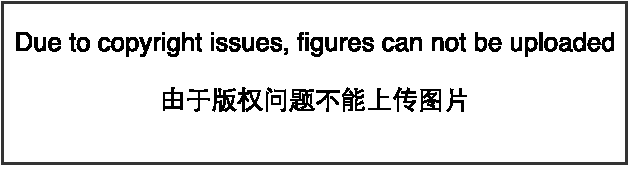
\includegraphics{figure.pdf}}
\else
	\centerline{\includegraphics{Chapter12/figures/gcn_sphere_color}}
\fi
	\caption{TODO}
	\label{fig:gcn_sphere_color}
\end{figure}


与直觉相反的是,存在被称为\firstgls{sphering}的预处理操作,并且它不同与\gls{GCN}。
\gls{sphering}并不会使数据位于球形壳上,而是将主要分量重新缩放以具有相等方差,使得\gls{PCA}使用的多变量正态分布具有球形等高线。 
\gls{sphering}通常被称为\firstgls{whitening}。
% 444 head


\gls{GCN}常常不能突出我们想要突出的图像特征,例如边缘和角。
如果我们有一个场景,有一个大的黑暗区域和一个大的明亮的区域(例如一个城市广场有一半的区域处于建筑物的阴影),
则\gls{GCN}将确保暗区域的亮度与亮区域的亮度之间存在大的差异。
然而,它不能确保暗区内的边缘突出。
% 444

这催生了\firstall{LCN} 。
\gls{LCN}确保对比度在每个小窗口上被归一化,而不是作为整体在图像上被归一化。
关于\gls{LCN}和\gls{GCN}的比较可以参考图\ref{fig:122}。
% 444
% src0    gray0, gcn0?   lcn0  
%    src1?  gcn1?  gray1?     lcn1  
\begin{figure}[!htb]
\ifOpenSource
\centerline{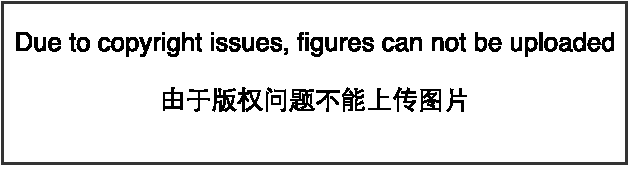
\includegraphics{figure.pdf}}
\else
	\centerline{\includegraphics{Chapter12/figures/src0}}
	\centerline{\includegraphics{Chapter12/figures/gcn0}}
	\centerline{\includegraphics{Chapter12/figures/lcn0}}	
	\centerline{\includegraphics{Chapter12/figures/src1}}
	\centerline{\includegraphics{Chapter12/figures/gcn1}}
	\centerline{\includegraphics{Chapter12/figures/lcn1}}				
\fi
	\caption{TODO}
	\label{fig:122}
\end{figure}

\gls{LCN}的各种定义都是可行的。
 在所有情况下,我们可以通过减去邻近像素的平均值并除以邻近像素的\gls{standard_deviation}来修改每个像素。
在一些情况下,要计算修改的像素为中心的矩形窗口中的所有像素的平均值和\gls{standard_deviation}\citep{Pinto08}。
在其他情况下,这是使用以要修改的像素为中心的高斯权重的加权平均和加权\gls{standard_deviation}。
在彩色图像的情况下,一些策略分别处理不同的颜色通道,而其他策略组合来自不同通道的信息以使每个像素标准化\citep{sermanet-icpr-12}。
% 444

\gls{LCN}通常可以通过使用可分离卷积(参见\ref{sec:efficient_convolution_algorithms}节)来计算\gls{feature_map}所需要的局部平均值和局部\gls{standard_deviation},然后使用元素层面的减法和元素层面的除法实现不同的\gls{feature_map}。
% 444

\gls{LCN}是可微分的操作,并且还可以用作应用于网络的隐藏层的非线性作用,以及应用于输入的预处理操作。
% 444

与\gls{GCN}一样,我们通常需要\gls{regularization}\gls{LCN}以避免除以零。
事实上,因为\gls{LCN}通常作用于较小的窗口,所以\gls{regularization}更加重要。
较小的窗口更可能包含彼此几乎相同的值,因此更可能具有零\gls{standard_deviation}。
% 445


\subsection{\glsentrytext{dataset_augmentation}}
\label{sec:dataset_augmentation_chap12}
如\ref{sec:chap7_dataset_augmentation}节中所讲到的,通过增加训练集的额外副本来增加训练集的大小,从而改进分类器的\gls{generalization}能力。
其中训练集的额外副本并不改变其标签。
对象识别是特别适合于这种形式的\gls{dataset_augmentation}的分类任务,因为标签对于许多变换是不变的,可以对输入使用许多几何变换。
如前所述,分类器可以受益于随机转换旋转,以及在某些情况下,输入的翻转以增强数据集。
 在专门的\gls{CV}应用中,更高级的变换通常用于\gls{dataset_augmentation}。
这些方案包括图像中颜色的随机扰动~\citep{Krizhevsky-2012},以及对输入的非线性几何变形~\citep{chapter-gradient-document-2001}。
% 445




\section{\glsentrytext{SR}}
\label{sec:speech_recognition}
% 446

\gls{SR}任务是将一段包括了自然语言发音的声音信号投影到对应的说话人的词序列上。
令$\MX=(\Vx^{(1)},\Vx^{(2)},\ldots,\Vx^{(T)})$表示语音的输入向量(传统做法是通过以20ms为一桢分割信号)。
许多\gls{SR}的系统通过特殊的手工设计的方法预处理输入信号,从而提取特征,但是某些\gls{DL}系统\citep{jaitly2011learning}直接从原始输入中学习特征。
令$\Vy=(y_{1},y_{2},\ldots,y_{N})$表示目标的输出序列(通常是一个词或者字符的序列)。
\firstall{ASR}任务指的是构造一个函数$f^*_{\text{ASR}}$,使得它能够在给定语音序列$\MX$的情况下计算最有可能的$\Vy$序列:
\begin{align}
\label{eqn:124}
f^*_{\text{ASR}}(\MX) =  \underset{\Vy}{\arg\max}  P^*(\Vy \vert \RMX = \MX)
\end{align}
其中$P^*$是给定输入值$\MX$时对应目标$\Vy$的条件分布。
% 446

从20世纪80年代直到2009-2012年,最先进的\gls{SR}系统是\firstall{HMM}和\firstall{GMM}的结合。
\glssymbol{GMM}对语音特征和\firstgls{phoneme}之间的关系建模\citep{Bahl87},\glssymbol{HMM}对\gls{phoneme}序列建模。
\glssymbol{GMM}-\glssymbol{HMM}模型将语音信号视作由如下过程生成:首先,一个\glssymbol{HMM}生成了一个\gls{phoneme}的序列以及离散的\gls{phoneme}子状态(比如每一个\gls{phoneme}的开始,中间,结尾),然后\glssymbol{GMM}把每一个离散的状态转化为一个简短的声音信号。
尽管直到最近\glssymbol{GMM}-\glssymbol{HMM}一直在\gls{ASR}中占据主导地位,\gls{SR}仍然是\gls{NN}所成功应用的第一个领域。
从20世纪80年代末期到90年代初期,许多的\gls{SR}系统使用了\gls{NN}\citep{Bourlard-cspla89,Waibel89b,Robinson+Fallside91,Bengio91z,Bengio92c,Konig96}。
在那段时间,基于\gls{NN}的\gls{ASR}的表现和\glssymbol{GMM}-\glssymbol{HMM}系统的表现差不多。
比如说,\citet{Robinson+Fallside91}在TIMIT数据集\citep{garofolo1993darpa}(有39个区分的\gls{phoneme})上达到了26\%的\gls{phoneme}错误率,这个结果优于或者是可比于基于\glssymbol{HMM}的结果。
从那时起,TIMIT成为了\gls{phoneme}识别的一个基准数据集,在\gls{SR}中的作用就和MNIST在图像中的作用差不多。
然而,由于\gls{SR}软件系统中的复杂的工程因素以及在基于\glssymbol{GMM}-\glssymbol{HMM}的系统中所已经付出的巨大努力,工业界并没有转向\gls{NN}。
结果,直到21世纪00年代末期,学术界和工业界的研究者们更多的是用\gls{NN}为\glssymbol{GMM}-\glssymbol{HMM}系统学习一些额外的特征。
% 447


之后,随着更大的更深的模型,更大的数据集的出现,通过使用\gls{NN}代替\glssymbol{GMM}来实现将语音的特征转化为\gls{phoneme}(或者\gls{phoneme}的子状态)可以大大的提高识别的精度。
从2009年开始,\gls{SR}的研究者们将一种\gls{unsupervised_learning}的\gls{DL}方法应用于\gls{SR}。
这种\gls{DL}方法基于训练一个被称作是\gls{RBM}的无向概率模型,从而对输入数据建模。
 \gls{RBM}将会在第三部分中被描述。
 为了完成\gls{SR}任务,\gls{unsupervised}的\gls{pretraining}被用来构造一个\gls{deep_feedforward_network},这个\gls{NN}是通过训练\gls{RBM}来初始化的。
 这些网络的输入是从一个固定规格的滑动窗(以当前桢为中心)的谱特征中抽取,预测了当前桢的条件概率。
 训练一个这样的\gls{NN}能够可以显著提高在TIMIT数据集上的识别率~\citep{mohamed2009deep,Mohamed+Dahl+Hinton-2012},并将\gls{phoneme}级别的错误率从26\%降到了20.7\%。
关于这个模型成功原因的详细分析可以参考\citet{mohamed2012understanding}。  
 对于基础\gls{SR}的扩展包括了添加自适应的说话人相关的特征\citep{mohamed2011deep}的方法,可以进一步的降低错误率。
 紧接着的工作是将结构从\gls{phoneme}识别(TIMIT所主要关注的)转向了大规模词汇语音识别\citep{Dahl2012},这不仅包含了识别\gls{phoneme},还包括了识别大规模词汇的序列。
\gls{SR}上的\gls{DNN}从最初的使用\gls{RBM}进行\gls{pretraining}发展到了使用\gls{ReLU}和\gls{dropout}等较为先进的技术~\citep{Zeiler+al-ICASSP-2013,Dahl-et-al-ICASSP2013}。
从那时开始,工业界的几个语音研究组开始寻求与学术圈的研究者之间的合作。
\citet{Hinton-et-al-2012}描述了这些合作所带来的突破性进展,这些技术现在在移动手机端广泛应用。
% 447

随后,当他们使用了越来越大的带标签的数据集,加入了各种初始化,训练方法以及调试\gls{DNN}的结构之后,他们发现这种\gls{unsupervised}的\gls{pretraining}方式是没有必要的,或者说不能带来任何显著的改进。
% 447

用\gls{SR}中词错误率来衡量,在\gls{SR}性能上的这些突破是史无前例的(大约30\%的提高),在这之前的长达十年左右的时间基于\glssymbol{GMM}-\glssymbol{HMM}的系统的传统技术已经停滞不前了,尽管数据集的规模是随时间增长的(见\citet{Deng+Yu-2014}的图2.4)。
这也导致了\gls{SR}领域快速的转向\gls{DL}的研究。
在大约的两年时间内,工业界的大多数的\gls{SR}产品都包含了\gls{DL},这种成功也激发了\gls{ASR}领域对\gls{DL}算法和结构的一波新的研究浪潮,并且影响至今。
% 448

其中的一个创新点是\gls{CNN}的应用\citep{Sainath-et-al-ICASSP2013}。
\gls{CNN} 在时间和频率维度复用了权重,改进了之前的仅对时间使用重复权值的\gls{TDNNs}。
这种新的二维的卷积模型并不是将输入的频谱当作一个长的向量,而是当成是一个图像,其中一个轴对应着时间,另一个轴对应的是谱分量的频率。
% 448

另一个重要的至今仍然活跃的推动,是完全抛弃了\glssymbol{HMM}的\firstgls{end_to_end}\gls{DL}\gls{SR}系统。
这个领域的第一个主要的突破是\citep{Graves-et-al-ICASSP2013},其中训练了一个深度的\gls{LSTM}的\gls{RNN}(见\ref{sec:the_long_short_term_memory_and_other_gated_rnns}节),使用了桢-\gls{phoneme}排列的\gls{MAP}估计推断,比如\citet{chapter-gradient-document-2001},以及CTC框架~\citep{Graves-et-al-2006,Graves-book2012}。
一个深度\gls{RNN}~\citep{Graves-et-al-ICASSP2013}在每一步都有状态变量,has state variables from several layers at each time step, giving the unfolded graph two kinds of depth: ordinary depth due to a stack of layers, and depth due to time unfolding
这个工作把TIMIT数据集上\gls{phoneme}的错误率降到了记录的新低17.7\%。关于应用于其它领域的深度\gls{RNN}的变种可以参考\citet{Pascanu-et-al-ICLR2014,Chung-et-al-NIPSDL2014-small}。
% 448

另一个\gls{end_to_end}\gls{DL}\gls{SR}的最新方法是让系统学习如何利用\firstgls{phonetic}层级的信息排列\firstgls{acoustic}层级的信息\citep{Chorowski-et-al-arxiv2014,llu_is2015b}。
% 448


% Translator: Shenjian Zhao
\section{\glsentrytext{NLP}}
\label{sec: natural_language_processing}

\firstgls{NLP} 让计算机使用人类语言,例如英语或法语。
计算机程序通常读取和发出专门的语言,让简单的程序能够高效和明确地解析。
而自然的语言通常是模糊的,并且会违背形式的描述。
\gls{NLP} 中的应用如机器翻译,学习者必须用一种人类语言读取句子并用另一种人类语言发出等同的句子。
许多\glssymbol{NLP}应用程序基于\gls{language_model},\gls{language_model}定义一个关于自然语言中的字,字符或字节序列的概率分布。

% -- 448 --

与本章讨论的其他应用一样,非常通用的\gls{NN}技术可以成功地应用于\gls{NLP}。
然而,为了实现卓越的性能并扩展到大型应用程序,一些领域特定的策略也很重要。
为了构建自然语言的有效模型,通常必须使用专门处理序列数据的技术。
在很多情况下,我们将自然语言视为一系列词,而不是单个字符或字节序列。
因为可能的词总数非常大,基于词的\gls{language_model}必须在极高维度和稀疏的离散空间上操作。
为使这种空间上的模型在计算和统计意义上都高效,研究者已经开发了几种策略。

\subsection{\glsentrytext{n_gram}}
\label{sec:n_grams}

\firstgls{language_model}定义了自然语言中的\gls{token}序列的概率分布。
根据模型的设计,\gls{token}可以是词、字符、甚至是字节。
\gls{token}总是离散的实体。
最早成功的\gls{language_model}基于固定长度序列的\gls{token}模型,称为\gls{n_gram}。
一个\gls{n_gram}是一个包含$n$个\gls{token}的序列。


基于\gls{n_gram}的模型定义给定前$n-1$个\gls{token}后的第$n$个\gls{token}的条件概率。
该模型使用这些条件分布的乘积来定义较长序列的概率分布:
\begin{align}
P(x_1, \dots, x_\tau) = P(x_1, \dots, x_{n-1}) \prod_{t=n}^\tau P(x_t \mid x_{t-n+1}, \dots, x_{t-1} ).
\end{align}
这个分解可以由概率的链式法证明。
初始序列 $P(x_1, \dots, x_{n-1})$的概率分布可以通过带有较小$n$值的不同模型来建模。

训练\gls{n_gram}模型是简单的,因为\gls{maximum_likelihood_estimation}可以简单地计算每个可能的\gls{n_gram}在训练集中出现的次数来计算。                                                                                                                                                                                                                                                                                                                                                                                       
几十年来,基于\gls{n_gram}的模型都是统计\gls{language_model}的核心模块~\citep{Jelinek+Mercer80,Katz87,Chen+Goodman99}。

对于小的$n$值,模型有特定的名称:$n=1$称为\firstgls{unigram},$n=2$称为\firstgls{bigram}及$n=3$称为\firstgls{trigram}。
这些名称源于相应数字的拉丁前缀和希腊后缀``-gram'',表示所写的东西。

% -- 449 --

通常我们同时训练\gls{n_gram}模型和$n-1$ gram模型。 
这使得它很容易计算概率:
\begin{align}
\label{eq:ml-ngram}
P(x_t \mid x_{t-n+1}, \dots, x_{t-1}) = \frac{P_n(x_{t-n+1}, \dots, x_t)} { P_{n-1}( x_{t-n+1}, \dots, x_{t-1}) }
\end{align}
简单地查找两个存储的概率就能计算。
为了在$P_n$中精确地再现\gls{inference},我们训练$P_{n-1}$时必须省略每个序列最后的字符。

举个例子,我们演示三元模型如何计算句子``{\tt THE DOG RAN AWAY}.''的概率。
句子的第一个词不能通过上述条件概率的公式计算,因为句子的开头没有上下文。
取而代之,在句子的开头我们必须使用词的边缘概率。
因此我们计算$P_3({\tt THE\ DOG\ RAN})$。
最后,可以使用条件分布$P({\tt AWAY} \mid {\tt DOG\ RAN})$(典型情况)来预测最后一个词。
将这与式\eqref{eq:ml-ngram}放在一起,我们得到:
\begin{align}
P({\tt THE\ DOG\ RAN\ AWAY}) = P_3({\tt THE\ DOG\ RAN}) P_3({\tt DOG\ RAN\ AWAY}) / P_2({\tt DOG\ RAN}).
\end{align}

\gls{n_gram}模型最大似然的基本限制是,在许多情况下从训练集计数估计的$P_n$很可能为零,即使元组$(x_{t-n+1},  \ldots, x_{t})$可能出现在测试集中。
这可能会导致两种不同的灾难性后果。
当$P_{n-1}$为零时,该比率是未定义的,因此模型甚至不能产生意义的输出。
当 $P_{n-1}$非零而$P_n$为零时,测试样本的对数似然为 $-\infty$。
为避免这种灾难性的后果,大多数\gls{n_gram}模型采用某种形式的\firstgls{smoothing}。
\gls{smoothing}技术将概率质量从观察到的元组转移到类似的未观察到的元组。
见\citet{Chen+Goodman99}的综述和实验比较。
其中一种基本技术基于向所有可能的下一个符号值添加非零概率质量。
这个方法可以被证明是,计数参数具有均匀或\ENNAME{Dirichlet}先验的贝叶斯\gls{inference}。
另一个非常流行的想法是包含高阶和低阶\gls{n_gram}模型的混合模型,其中高阶模型提供更多的\gls{capacity},而低阶模型尽可能地避免零计数。
如果上下文$x_{t-n+k}, \ldots, x_{t-1}$的频率太小而不能使用高阶模型,\textbf{回退方法}(back-off methods)就查找低阶\gls{n_gram} 。
更正式地说,它们通过使用上下文$x_{t-n+k}, \ldots, x_{t-1}$来估计$x_t$上的分布,并增加$k$直到找到足够可靠的估计。
有 $|\SetV|^n$ 可能的\gls{n_gram}, 而且 $|\SetV|$ 通常很大。
% -- \450 --

经典的\gls{n_gram}模型特别容易引起\gls{curse_of_dimensionality}。
即使有大量训练数据和适当的$n$,大多数\gls{n_gram}也不会出现在训练集中。
经典\gls{n_gram}模型的一种观点是执行最近邻查询。
换句话说,它可以被视为局部\gls{nonparametric}预测器,类似于$k$-最近邻。
这些极端局部预测器面临的统计问题在\ref{sec:local_constancy_and_smoothness_regularization}节中描述。
\gls{language_model}的问题甚至比普通模型更严重,因为任何两个不同的词在\gls{one_hot}向量空间中具有彼此相同的距离。
因此,难以大量利用来自任意``邻居''的信息 —— 只有重复相同上下文的训练样本对局部泛化有用。
为了克服这些问题,\gls{language_model}必须能够在一个词和其他语义相似的词之间共享知识。
为了提高\gls{n_gram}模型的统计效率,\textbf{基于类的语言模型}(class-based language model)~\citep{Brown92,Ney+Kneser93,Niesler98}引入词类别的概念,然后属于同一类别的词共享词之间的统计强度。
这个想法使用聚类算法,基于它们与其他词同时出现的频率,将该组词分成集群或类。
随后,模型可以在条件竖杠的右侧使用词类ID而不是单个词ID。
混合(或回退)词模型和类模型的复合模型也是可能的。
尽管词类提供了在序列之间泛化的方式,但其中一些词被相同类的另一个替换,导致该\gls{representation}丢失了很多信息。

\subsection{\glsentrytext{NLM}}
\label{sec:neural_language_models}

\firstall{NLM}是一类设计用来克服\gls{curse_of_dimensionality}的\gls{language_model},它使用词的\gls{distributed_representation}对自然语言序列建模~\citep{BenDucVin01-small}。
不同于基于类\gls{n_gram}模型,\gls{NLM}在识别两个相似的词的基础上,而不丧失将每个词编码为彼此不同的能力。
\gls{NLM}共享一个词(及其上下文)和其他类似词(和上下文之间)的统计强度。
模型为每个词学习的\gls{distributed_representation},允许模型处理具有类似共同特征的词来实现这种共享。
例如,如果词{\tt dog}和词{\tt cat}映射到具有许多属性的表示,则包含词{\tt cat}的句子可以告知模型对包含词{\tt dog}的句子做出预测,反之亦然。
因为这样的属性很多,所以存在许多泛化的方式,可以将信息从每个训练语句传递到指数数量的语义相关语句。
\gls{curse_of_dimensionality}需要模型泛化到相对句子长度是指数多的句子。
该模型通过将每个训练句子与指数数量的类似句子相关联来克服这个问题。

% -- 451 --

我们有时将这些词\gls{representation}称为\firstgls{word_embedding}。
在这个解释下,我们将原始符号视为维度等于词表大小的空间中的点。
词\gls{representation}将这些点嵌入到较低维的特征空间中。
在原始空间中,每个词由一个\gls{one_hot}向量表示,因此每对词彼此之间的欧氏距离都是$\sqrt{2}$。
在嵌入空间中,经常出现在类似上下文(或共享由模型学习的一些``特征''的任何词对)中的词彼此接近。
这通常导致具有相似含义的词变得邻近。
图\ref{fig:chap12_word_embeddings_color}放大了学到的\gls{word_embedding}空间的特定区域,我们可以看到语义上相似的词如何映射到彼此接近的表示。

\begin{figure}[htp]
\centering
\ifOpenSource
\centerline{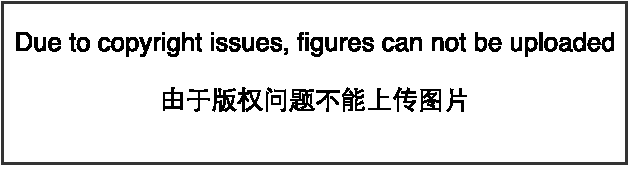
\includegraphics{figure.pdf}}
\else
\includegraphics{Chapter12/figures/word_embeddings_color.pdf}
\fi
\caption{TODO}
\label{fig:chap12_word_embeddings_color}
\end{figure}

也有其他领域的\gls{NN}定义嵌入。
例如,\gls{convolutional_network}的隐藏层提供``图像嵌入''。
通常\glssymbol{NLP}从业者对嵌入的这个想法更感兴趣,因为自然语言最初不在于实值向量空间。
隐藏层在表示数据的方式上提供了更质变的戏剧性变化。

% -- 452 --

使用\gls{distributed_representation}来改进\gls{NLP}模型的基本思想不用局限于\gls{NN}。
它还可以用于\gls{graphical_model},其中\gls{distributed_representation}基于多个隐变量形式。

\subsection{高维输出}
\label{sec:high_dimensional_outputs}

在许多自然语言应用中,我们经常希望我们的模型产生词(而不是字符)作为输出的基本单位。
对于大词汇表,由于词汇量很大,在词的选择上表示输出分布计算上可能是昂贵的。
在许多应用中,$\SetV$包含数十万词。
表示这种分布的朴素方法是应用一个仿射变换,将隐藏表示转换到输出空间,然后应用\ENNAME{softmax}函数。
假设我们的词汇表$\SetV$大小为$| \SetV |$。
因为其输出维数为$| \SetV |$,描述该仿射变换线性分量的权重矩阵非常大。
这增加了表示该矩阵的高存储成本,以及乘以它的高计算成本。
因为\ENNAME{softmax}在所有$| \SetV |$输出之间归一化,所以在训练时以及测试时执行全矩阵乘法是必要的 ——我们不能仅计算与正确输出的权重向量的点积。
因此,输出层的高计算成本在训练期间(计算似然性及其梯度)和测试期间(计算所有或所选词的概率)同时出现。
对于专门的\gls{loss_function},可以有效地计算梯度 \citep{Vincent2015},但是应用于传统\ENNAME{softmax}输出层的标准\gls{cross_entropy}损失时会出现了许多困难。

假设$\Vh$是用于预测输出概率$\hat \Vy$的顶部隐藏层。
如果我们用学到的权重$\MW$和学到的\gls{bias_aff}$\Vb$来参数化从$\Vh$到$\hat \Vy$的变换,则仿射\ENNAME{softmax}输出层执行以下计算:
\begin{align}
\label{eq:softmax-over-words}
  a_i &= b_i + \sum_j  W_{ij} h_j \;\;\; \forall i \in \{1,\ldots,|\SetV|\}, \\
  \hat{y}_i &= \frac{e^{a_i}}{\sum_{i'=1}^{|\SetV|} e^{a_{i'}}}.
\end{align}
如果$\Vh$包含$n_h$个元素,则上述操作复杂度是 $O(|\SetV| n_h)$。
$n_h$为数千和$| \SetV |$数十万的情况下,这个操作占据了\gls{NLM}的大多数计算。

% -- 453 --

\subsubsection{使用\glsentrytext{shortlist}}
第一个\gls{NLM}\citep{BenDucVin01-small,Bengio-nnlm2003-small}通过将词汇量限制为10,000或20,000来减轻大词汇表上\ENNAME{softmax}的高成本。
\citet{Schwenk+Gauvain2002}和 \citet{Schwenk-2007}在这种方法的基础上建立新的方式,将词汇表$\SetV$分为最常见词汇(由\gls{NN}处理)的\firstgls{shortlist}~$\SetL$和较稀有词汇的尾列表$\SetT = \SetV \backslash \SetL$(由\gls{n_gram}模型处理)。
为了组合这两个预测,\gls{NN}还必须预测在上下文$C$之后出现的词位于尾部列表的概率。
可以添加额外的\ENNAME{sigmoid}输出单元估计 $P(i \in \SetT \mid C)$实现这个预测。
额外输出则可以用来估计$\SetV$中所有词的概率分布,如下:
\begin{align}
 P(y=i\mid C)  =& 1_{i \in \SetL} P(y=i\mid C, i \in \SetL) (1 - P(i \in \SetT\mid C)) \nonumber \\
     & + 1_{i \in \SetT} P(y=i\mid C, i \in \SetT) P(i \in \SetT\mid C),
\end{align}
其中$P(y=i\mid C, i \in \SetL)$由\gls{NLM}提供$P(y=i\mid C, i \in \SetT)$由\gls{n_gram}模型提供。
稍作修改,这种方法也可以在\gls{NLM}模型的\ENNAME{softmax}层中使用额外的输出值,而不是单独的\ENNAME{sigmoid}单元。

\gls{shortlist}方法的一个明显的缺点是,\gls{NLM}模型的潜在泛化优势仅限于最常用的词,这大概是最没用的。
这个缺点激发了处理高维输出替代方法的探索,如下所述。

\subsubsection{分层Softmax}
减少大词汇表$\SetV$上高维输出层计算负担的经典方法~\citep{Goodman2001}是分层地分解概率。
无需与$|\SetV|$成比例数量 (并且也与隐藏单元数量$n_h$成比例)的计算,$|\SetV|$因子可以降低到$\log |\SetV|$一样低。
\citet{BengioTR1215}和\citet{Morin+Bengio-2005-small} 将这种因子分解方法引入\gls{NLM}中。

% -- 454 --

我们可以认为这种层次结构是先建立词的类别,然后是词类别的类别,然后是词类别的类别的类别,等等
这些嵌套类别构成一棵树,其叶上是词。
在平衡树中,树的深度为$\log |\SetV|$。
选择一个词的概率是由路径(从树根到包含该词叶子的路径)上的每个节点通向该词分支概率的乘积给出。
图\ref{chap12_word_hierarchy}是一个简单的例子。
\citet{Mnih+Hinton-2009}也描述了使用多个路径来识别单个词的方法,以便更好地建模具有多个含义的词。
计算词的概率则涉及在导向该词所有路径上的求和。
\begin{figure}[htp]
\centering
\ifOpenSource
\centerline{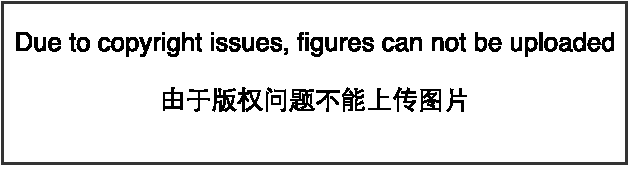
\includegraphics{figure.pdf}}
\else
\includegraphics{Chapter12/figures/word_hierarchy.pdf}
\fi
% Magic incantation to allow math in caption
\captionsetup{singlelinecheck=off}
% Part of the incantation is that we must define the [] argument
\caption{TODO}
\label{fig:chap12_word_hierarchy}
\end{figure}
\begin{align}
    \text{TODO Equation in Figure}  \\
    \text{TODO Equation in Figure}
\end{align}

为了预测树的每个节点所需的条件概率,我们通常在树的每个节点处使用\gls{logistic_regression}模型,并且为所有这些模型提供与输入相同的上下文$C$。
因为正确的输出被编码在训练集中,我们可以使用\gls{supervised_learning}训练\gls{logistic_regression}模型。
通常使用标准\gls{cross_entropy}损失,对应于最大化正确判断序列的对数似然。

因为可以高效地计算输出对数似然(低至$\log |\SetV|$而不是$ |\SetV|$),所以也可以高效地计算梯度。
不仅包括关于输出参数的梯度,而且还包括关于隐藏层激活的梯度。

优化树结构最小化期望的计算数量是可能的,但通常不实际。
给定词的相对频率,信息理论的工具可以指定如何选择最佳二进制代码。
为此,我们可以构造树,使得与词相关联的位数量近似等于该词频率的对数。
然而在实践中,节省计算通常不值得努力,因为输出概率的计算仅是\gls{NLM}中总计算的一部分。
例如,假设有$l$个全连接的宽度为$n_h$的隐藏层。
令$n_b$是识别一个词所需比特数的加权平均值,其加权由这些词的频率给出。
在这个例子中,计算隐藏激活所需的操作数增长为$O(ln_h^2)$,而输出计算增长为$O(n_h n_b)$。
只要$ n_b \leq l n_h$,我们可以通过收缩$n_h$比收缩$n_b$减少更多的计算量。
事实上,$n_b$通常很小。
因为词汇表的大小很少超过一百万而$\log_ 2(10^6) \approx 20$,所以可以将$n_b$减小到大约20,但$n_h$通常大得多,大约为$10^3$或更大。
我们可以定义深度为2和分支因子为$\sqrt{|\SetT|}$的树,而不用仔细优化分支因子为$2$的树。
这样的树对应于简单定义一组互斥的词类。
基于深度为$2$的树的简单方法可以获得层级策略大部分的计算益处。

% -- 455 --

一个仍然有点开放的问题是如何最好地定义这些词类,或者如何定义一般的词层次结构。
早期工作使用现有的层次结构\citep{Morin+Bengio-2005-small} ,但也可以理想地与\gls{NLM}联合学习层次结构。
学习层次结构很困难。
对数似然的精确优化似乎难以解决,因为词层次的选择是离散的,不适于基于梯度的优化。
然而,可以使用离散优化来近似地最优化词类的分割。

分层\ENNAME{softmax}的一个重要优点是,它在训练期间和测试期间(如果在测试时我们想计算特定词的概率)都带来了计算的好处。

当然即使使用分层\ENNAME{softmax},计算所有$|\SetT|$词的概率仍将是昂贵的。
另一个重要的操作是在给定上下文中选择最可能的词。
不幸的是,树结构不能为这个问题提供有效和精确的解决方案。

缺点是在实践中,分层\ENNAME{softmax}倾向于更差的测试结果(相对基于采样的方法),我们将在下面描述。
这可能是词类选择得不好。

\subsubsection{\glsentrytext{importance_sampling}}
加速\gls{NLM}训练的一种方式是避免明确计算所有词(未出现在下一位置)对梯度的贡献。
每个不正确的词在此模型下应该具有低概率。
枚举所有这些单词计算成本可能会很高。
相反,可以仅采样词的子集。
使用式\eqref{eq:softmax-over-words}中引入的符号,梯度可以写成如下形式:
\begin{align}
 \frac{\partial \log P(y \mid C)}{\partial \theta} &= \frac{\partial \log {\rm softmax}_y(\Va)}{\partial \theta} \\ 
  &= \frac{\partial}{\partial \theta} \log \frac{e^{a_y}}{\sum_i e^{a_i}} \\ 
 &= \frac{\partial}{\partial \theta} (a_y - \log \sum_i e^{a_i}) \\ 
 &= \frac{\partial a_y}{\partial \theta}  - \sum_i P(y = i \mid C) \frac{\partial a_i}{\partial \theta},
\end{align}
其中$\Va$是\ENNAME{presoftmax}激活(或分数)向量,每个词对应一个元素。
第一项是\textbf{正相}(positive phase)项推动$a_y$向上,而第二项是\textbf{负相}(negative phase)项,对于所有$i$以权重$P(i \mid C)$推动$a_i$向下。
由于负相项是期望值,我们可以用\gls{monte_carlo}采样来估计。
然而,这将需要从模型本身采样。
从模型中抽样需要对词汇表中所有的$i$计算$P(i \mid C)$,这正是我们试图避免的。

我们可以从另一个分布中抽样,而不是从模型中抽样,称为\firstgls{proposal_distribution}(记为$q$),并通过适当的权重来校正从错误分布抽样引入的\gls{bias_sta} \citep{Bengio+Senecal-2003-small,Bengio+Senecal-2008}。
这是一种称为\firstgls{importance_sampling}的更通用技术的应用,我们将在\ref{sec:importance_sampling}节中更详细地描述。
不幸的是,即使精确\gls{importance_sampling}也不一定有效,因为需要计算权重$p_i / q_i$,其中的$p_i = P(i \mid C)$只能在计算所有得分$a_i$后才能计算。
这个应用采取的解决方案称为\gls{biased_importance_sampling},其中重要性权重被归一化加和为1。
当对负词$n_i$进行采样时,相关联的梯度被加权为:
\begin{align}
  w_i = \frac{p_{n_i} / q_{n_i}}{\sum_{j=1}^N p_{n_j} / q_{n_j}}.
\end{align}
这些权重用于对来自$q$的$m$个负样本给出适当的重要性,以形成负相估计对梯度的贡献:
\begin{align}
  \sum_{i=1}^{|\SetV|} P(i \mid C) \frac{\partial a_i}{\partial \theta}  \approx \frac{1}{m} \sum_{i=1}^m w_i \frac{\partial a_{n_i}}{\partial \theta}.
  \end{align}
  \gls{unigram}或\gls{bigram}分布与\gls{proposal_distribution}$q$工作得一样好。
很容易从数据估计这种分布的参数。
在估计参数之后,也可以非常高效地从这样的分布采样。

\firstgls{importance_sampling}不仅可以加速具有较大\ENNAME{softmax}输出的模型。
更一般地,它可以加速具有大稀疏输出层的训练,其中输出是稀疏向量而不是$n$选$1$。
其中一个例子是\gls{bag_of_words}。
\gls{bag_of_words}具有稀疏向量$\Vv$,其中$v_i$表示词汇表中的词$i$存不存在文档中。
或者,$v_i$可以指示词$i$出现的次数。
由于各种原因,训练产生这种稀疏向量的\gls{ML}模型可能是昂贵的。
在学习的早期,模型可能不会真的使输出真正稀疏。
此外,将输出的每个元素与目标的每个元素进行比较,可能是描述用于训练的\gls{loss_function}可能最自然的方式。
这意味着稀疏输出并不一定能带来计算上的好处,因为模型可以选择使大多数输出非零,并且所有这些非零值需要与相应的训练目标进行比较( 即使训练目标是零)。
\citet{Dauphin2011-small} 证明可以使用\gls{importance_sampling}加速这种模型。
高效算法最小化``正词''(在目标中非零的那些词)和相等数量的``负词''的重构损失。
随机选择负词,如使用启发式抽样更可能被误解的词。
该启发式过采样引入的偏差则可以使用重要性权重校正。

% -- 458 --

在所有这些情况下,输出层梯度估计的计算复杂度被减少为与负样本数量成比例,而不是与输出向量的大小成比例。


\subsubsection{噪声对比估计和排名损失}


\label{sec:combining_neural_language_models_with_n_grams}
为减少训练大词汇表的\gls{NLM}计算成本,研究者也提出了其他基于抽样的方法。
早期的例子是 \citet{Collobert+Weston-ICML2008}提出的排名损失,将\gls{NLM}每个词的输出视为一个分数,并试图使正确词的分数$a_y$比其他词$a_i$排名更高。提出的排名损失则是
\begin{align} 
 L = \sum_i \max(0,1-a_y+a_i).
\end{align} 
如果观察到词的分数$a_y$远超过负词的分数$a_i$(相差大于1),则第$i$项梯度为零。
这个\gls{criterion}的一个问题是它不提供估计的条件概率,条件概率在很多应用中是有用的,包括语音识别和文本生成(包括诸如翻译的条件文本生成任务)。

最近用于\gls{NLM}的训练目标是噪声对比估计,将在\ref{sec:noise_contrastive_estimation}节中介绍。
这种方法已成功应用于\gls{NLM}\citep{Mnih+Teh-ICML2012,Mnih2013}。

% -- 459 --

\subsection{结合\glsentrytext{n_gram}和\glsentrytext{NLM}}
\gls{n_gram}模型相对\gls{NN}的主要优点是\gls{n_gram}模型具有更高的模型\gls{capacity}(通过存储非常多的元组的频率),并且处理样本只需非常少的计算量(通过查找只匹配当前上下文的几个元组)。
如果我们使用哈希表或树来访问计数,那么用于\gls{n_gram}的计算量几乎与\gls{capacity}无关。
相比之下,将\gls{NN}的参数数目加倍通常也大致加倍计算时间。
<BAD>例外包括避免每次计算时使用所有参数的模型。
嵌入层每次只索引单个嵌入,所以我们可以增加词汇量,而不增加每个样本的计算时间。
一些其他模型,例如平铺\gls{convolutional_network},可以在减少\gls{parameter_sharing}程度的同时添加参数以保持相同的计算量。然而,基于矩阵乘法的典型\gls{NN}层需要与参数数量成比例的计算量。

因此,增加\gls{capacity}的一种简单方法是将两种方法结合,由\gls{NLM}和\gls{n_gram}\gls{language_model}组成\gls{ensemble}~\citep{BenDucVin01-small,Bengio-nnlm2003-small}。

对于任何\gls{ensemble},如果\gls{ensemble}成员产生独立的错误,这种技术可以减少测试误差。
\gls{ensemble}的领域提供了许多方法来组合\gls{ensemble}成员的预测,包括统一加权和在验证集上选择权重。
\citet{Mikolov-Interspeech-2011} 扩展了\gls{ensemble},不仅包括两个模型,而包括大量模型。
也可以将\gls{NN}与最大熵模型配对并联合训练\citep{Mikolov-ASRU-2011}。
该方法可以被视为训练具有一组额外输入的\gls{NN},额外输入直接连接到输出并且不连接到模型的任何其他部分。
额外输入是输入上下文中特定\gls{n_gram}是否存在的指示器,因此这些变量是非常高维且非常稀疏的。

模型\gls{capacity}的增加是巨大的 (架构的新部分包含高达$| sV |^n$个参数 ),但是处理输入所需的额外计算量是很小的(因为额外输入非常稀疏)。

\subsection{\glsentrytext{NMT}}
\label{sec:neural_machine_translation}

机器翻译以一种自然语言读取句子并产生等同含义的另一种语言的句子。
机器翻译系统通常涉及许多组件。
在高层次,一个组件通常会提出许多候选翻译。
由于语言之间的差异,这些翻译中的许多翻译将是不符合语法的。
例如,许多语言在名词后放置形容词,因此直接翻译成英语时,它们会产生诸如``apple red''的短语。
提议机制提出建议翻译的许多变体,理想地应包括``red apple''。
翻译系统的第二个组成部分,\gls{language_model},评估提议的翻译,并可以评分``red apple''比``apple red''更好。

% -- 460 --

<BAD>最早的机器翻译\gls{NN}探索中已经纳入了\gls{encoder}和\gls{decoder}的想法(Allen 1987; Chrisman 1991; Forcada
and Ñeco 1997),而翻译中\gls{NN}的第一个大规模有竞争力的用途是通过\gls{NLM}升级翻译系统的\gls{language_model}~\citep{Schwenk-et-al-IWSLT2006,Schwenk-2010}。
之前,大多数机器翻译系统在该组件使用\gls{n_gram}模型。
机器翻译中基于\gls{n_gram}的模型不仅包括传统的回退\gls{n_gram}模型,而且包括\textbf{最大熵语言模型}(maximum entropy language models),其中给定上下文中常见的词affine-softmax层预测下一个词。

传统\gls{language_model}仅仅报告自然语言句子的概率。
因为机器翻译涉及给定输入句子产生输出句子,所以将自然\gls{language_model}扩展为有条件的是有意义的。
如\ref{sec:learning_conditional_distributions_with_maximum_likelihood}节所述可以直接地扩展一个模型,该模型定义某些变量的边缘分布,以便在给定上下文$C$($C$可以是单个变量或变量列表)的情况下定义该变量的条件分布。
\citet{Devlin-et-al-ACL2014}在一些统计机器翻译的基准中击败了最先进的技术,他给定源语言中短语$\RSs_1, \RSs_2,\ldots, \RSs_k$后使用\glssymbol{MLP}对目标语言的短语$\RSt_1, \RSt_2,\ldots, \RSt_k$进行评分。
这个\glssymbol{MLP}估计$P(\RSt_1, \RSt_2,\ldots, \RSt_k \mid \RSs_1, \RSs_2,\ldots, \RSs_k)$。
这个\glssymbol{MLP}的估计替代了条件\gls{n_gram}模型提供的估计。

基于\glssymbol{MLP}方法的缺点是需要将序列预处理为固定长度。
为了使翻译更加灵活,我们希望使用允许输入长度可变和输出长度可变的模型。
\glssymbol{RNN}具备这种能力。

\ref{sec:modeling_sequences_conditioned_on_context_with_rnns}节描述了给定某些输入后,关于序列条件分布的\glssymbol{RNN}的几种构造方法,并且\ref{sec:encoder_decoder_sequence_to_sequence_architectures}节描述了当输入是序列时如何实现这种条件分布。
在所有情况下,一个模型首先读取输入序列并产生概括输入序列的数据结构。我们称这个概括为``上下文''$C$。
上下文$C$可以是向量列表,或者向量或张量。
读取输入以产生$C$的模型可以是\glssymbol{RNN}\citep{Cho-et-al-EMNLP2014,Sutskever-et-al-NIPS2014,Jean-et-al-arxiv2014}或\gls{convolutional_network}\citep{Kalchbrenner+Blunsom-EMNLP2013}。
第二模型(通常是RNN),则读取上下文$C$并且生成目标语言的句子。
在图\ref{fig:chap12_encoder_decoder_architecture}中示出了这种用于机器翻译的\gls{encoder} - \gls{decoder}框架的总体思想。

% -- 461 --

\begin{figure}[htp]
\ifOpenSource
\centerline{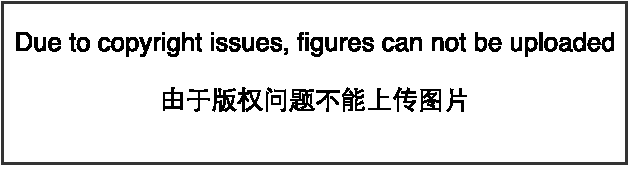
\includegraphics{figure.pdf}}
\else
\centerline{\includegraphics{Chapter12/figures/encoder_decoder_architecture.pdf}}
\fi
\caption{TODO}
\label{fig:chap12_encoder_decoder_architecture}
\end{figure}

为生成以源句为条件的整句,模型必须具有表示整个源句的方式。 
早期模型只能表示单个词或短语。
从\gls{representation_learning}的观点来看,具有相同含义的句子具有类似\gls{representation}是有用的,无论它们是以源语言还是以目标语言书写。
首先使用卷积和\glssymbol{RNN}的组合来探索该策略~\citep{Kalchbrenner+Blunsom-EMNLP2013}。
后来的工作介绍了使用\glssymbol{RNN}对所提议的翻译进行打分\citep{Cho-et-al-EMNLP2014}或生成翻译句子\citep{Sutskever-et-al-NIPS2014}。
\cite{Jean-et-al-arxiv2014} 将这些模型扩展到更大的词汇表。

% -- 462 --

\subsubsection{使用\glsentrytext{attention_mechanism}并对齐数据片段}
 使用固定大小的表示来概括非常长的句子(例如60个词)的所有语义细节是非常困难的。 
 这可以使用足够大的RNN,并且用足够长时间训练得很好,才能实现,如 \citet{Cho-et-al-EMNLP2014}和\citet{Sutskever-et-al-NIPS2014}所表明的。
 然而,更高效的方法是先读取整个句子或段落(以获得正在表达的上下文和焦点),然后一次翻译一个词,每次聚焦于输入句子的不同部分来收集产生下一个输出词所需的语义细节。
 这正是~\citet{Bahdanau-et-al-ICLR2015-small} 第一次引入的想法。
 图\ref{fig:chap12_attention}中展示了\gls{attention_mechanism},其中每个\gls{time_step}关注输入序列的特定部分。

 \begin{figure}[htp]
\ifOpenSource
\centerline{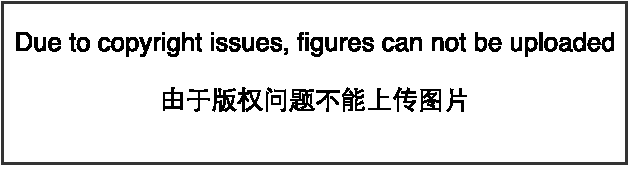
\includegraphics{figure.pdf}}
\else
\centerline{\includegraphics{Chapter12/figures/attention.pdf}}
\fi
\caption{TODO}
\label{fig:chap12_attention}
\end{figure}

我们可以认为基于\gls{attention_mechanism}的系统有三个组件:
\begin{itemize}
 \item   读取器 \emph{读取}原始数据(例如源语句中的源词)并将其转换为\gls{distributed_representation},其中一个特征向量与每个词的位置相关联。
 \item 存储器存储读取器输出的特征向量列表。这可以被理解为包含事实序列的\emph{存储器},而之后不必以相同的顺序从中检索,也不必访问全部。
 \item 最后一个程序\emph{利用}存储器的内容来顺序地执行任务,每个\gls{time_step}能聚焦于某个存储器元素的内容(或几个,具有不同权重)。
\end{itemize}
第三组件生成翻译语句。

% -- 463 --

当用一种语言书写的句子中的词与另一种语言的翻译语句中的相应词对齐时,可以使对应的\gls{word_embedding}相关联。
早期的工作表明,我们可以学习将一种语言中的\gls{word_embedding}与另一种语言中的\gls{word_embedding}相关联的翻译矩阵\citep{Kocisky-et-al-ACL2014},与传统的基于短语表中频率计数的方法相比,可以产生较低的对齐错误率。
甚至更早的工作\citep{Klementiev-et-al-COLING2012}研究跨语言词向量。 
这种方法的存在很多扩展。
例如,允许在更大数据集训练的更高效的跨语言对齐~\citep{Gouws-et-al-arxiv2014} 。

\subsection{历史观点}
\label{sec:historical_perspective_chap12}

<BAD>在\gls{back_propagation}的第一次探索中,\citet{Rumelhart86b-small}等人提出了\gls{distributed_representation}符号的思想,其中符号对应于族成员的身份,而\gls{NN}捕获族成员之间的关系,训练样本形成三元组如(Colin,Mother,Victoria)。
\gls{NN}的第一层学习每个族成员的表示。例如,Colin的特征可能代表Colin所在的族树,他所在树的分支,他来自哪一代等等。
我们可以将\gls{NN}认为是将这些属性关联在一起的计算学习规则,可以获得期望预测。
模型则可以进行预测,例如推断谁是Colin的母亲。

\cite{Deerwester90}将符号嵌入的想法扩展对词的嵌入。
这些嵌入使用SVD学习。 
之后,嵌入将通过\gls{NN}学习。

\gls{NLP}的历史是由流行表示(对模型输入不同方式的表示)的变化标志的  。
在早期对符号和词建模的工作之后,\gls{NN}在\glssymbol{NLP}上一些最早的应用\citep{Miikkulainen91,Schmidhuber96}将输入表示为字符序列。

\citet{BenDucVin01-small} 将焦点重新引到建模词并引入\gls{NLM},能产生可解释的\gls{word_embedding}。
这些神经模型已经从在一小组符号上的定义表示(20世纪80年代)扩展到现代应用中的数百万字(包括专有名词和拼写错误)。
这种计算扩展的努力导致了\ref{sec:high_dimensional_outputs}节中描述的技术发明。

% -- 464 --

最初,使用词作为\gls{language_model}的基本单元可以改进语言建模的性能 \citep{BenDucVin01-small}。
而今,新技术不断推动基于字符 \citep{Sutskever-et-al-ICML2011})和基于词的模型向前发展,最近的工作 \citep{gillick2015multilingual}甚至建模Unicode字符的单个字节。

\gls{NLM}背后的思想已经扩展到多个\gls{NLP}应用,如解析\citep{Henderson-NAACL2003,Henderson-ACL2004,Collobert-AISTATS2011},词性标注,语义角色标注,分块等,有时使用共享\gls{word_embedding}的单一多任务学习架构\citep{Collobert+Weston-ICML2008,collobert2011natural}。

<BAD>随着t-SNE\gls{dimensionality_reduction}算法的发展\citep{VanDerMaaten08-small},用于分析\gls{language_model}嵌入的二维可视化成为一种流行的工具,以及Joseph Turian在2009年引入的专用于可视化词嵌入的应用。

\section{其他应用}
\label{sec:other_applications}

在本节中,我们介绍\gls{DL}一些其他类型的应用,它们与上面讨论的标准对象识别、语音识别和\gls{NLP}任务不同。
本书的第三部分将扩大这个范围,甚至进一步扩展到仍是目前主要研究领域的任务。


\subsection{\glsentrytext{recommender_system}}
\label{sec:recommender_systems}
信息技术部门中\gls{ML}的主要应用之一是向潜在用户或客户推荐项目。
可以分为两种主要的应用:在线广告和项目建议(通常这些建议的目的仍然是为了销售产品)。
两者都依赖于预测用户和项目之间的关联, 如果展示了广告或向该用户推荐了该产品,\gls{recommender_system}要么预测一些行为的概率(用户购买产品或该行为的一些代替)或预期增益(其可取决于产品的价值)。
目前,互联网的资金主要来自于各种形式的在线广告。
经济的主要部分依靠网上购物。 
包括Amazon和eBay在内的公司使用\gls{ML}(包括\gls{DL})推荐他们的产品。
有时,项目不是实际出售的产品。
如选择在社交网络新闻信息流上显示的帖子、推荐观看的电影、推荐笑话、推荐专家建议、匹配视频游戏的玩家或匹配约会的人。

% -- 465 --
通常,这种关联问题像\gls{supervised_learning}问题一样处理:给出一些关于项目和关于用户的信息,预测感兴趣的行为(用户点击广告、输入评级、点击``喜欢''按钮、 购买产品,在产品上花钱、花时间访问产品页面等)。
通常这最终会归结到回归问题(预测一些条件期望值)或概率分类问题(预测一些离散事件的条件概率)。

早期\gls{recommender_system}的工作依赖于作为这些预测输入的最小信息:用户ID和项目ID。
在这种情况下,唯一的推广方式是依赖于不同用户或不同项目的目标变量值之间的模式相似性。
假设用户1和用户2都喜欢项目A,B和C.
由此,我们可以推断出用户1和用户2具有类似的口味。
如果用户1喜欢项目D,那么这可以强烈提示用户2也喜欢D。
基于此原理的算法称为\firstgls{collaborative_filtering}。
非参数方法(例如基于估计偏好模式之间相似性的最近邻方法)和参数方法都可能用来解决这个问题。
参数方法通常依赖于为每个用户和每个项目学习\gls{distributed_representation}(也称为嵌入)。
目标变量的双线性预测(例如评级)是一种简单的参数方法,这种方法非常成功,通常被认为是最先进系统的组成部分。
通过用户嵌入和项目嵌入之间的点积(可能需要通过仅依赖于用户ID或项目ID的常数来校正)获得预测。
令$\hat{\MR}$是包含我们预测的矩阵,$\MA$矩阵行中是用户嵌入,$\MB$矩阵列中具有项目嵌入。
令$\Vb$和$\Vc$是分别包含针对每个用户(表示用户平常坏脾气或积极的程度)以及每个项目(表示其大体受欢迎程度)的\gls{bias_aff}向量。
因此,双线性预测如下获得:
\begin{equation}
\label{eq:bilinear-prediction}
 \hat{R}_{u,i} = b_u + c_i + \sum_j A_{u,j} B_{j,i}.
\end{equation}
通常,人们希望最小化预测评级$\hat{R}_{u,i}$ 和实际评级$\hat{R}_{u,i}$ 之间的平方误差。
当用户嵌入和项目嵌入首次缩小到低维度(两个或三个)时,它们就可以方便地可视化,或者可以用于将用户或项目彼此进行比较(就像\gls{word_embedding})。
获得这些嵌入的一种方式是对实际目标(例如评级)的矩阵$\MR$进行\gls{SVD}。
这对应于将$\MR = \MU \MD \MV'$(或归一化的变体)分解为两个因子的乘积,低秩矩阵 $\MA=\MU \MD$ and $\MB = \MV'$。
\glssymbol{SVD}的一个问题是它以任意方式处理丢失的条目,如同它们对应于目标值0。
相反,我们希望避免为缺失条目做出的预测付出任何代价。
幸运的是,观察到的评级的平方误差总和也可以通过基于梯度的优化最小化。
\glssymbol{SVD}和式 \eqref{eq:bilinear-prediction}中的双线性预测在\ENNAME{Netflix}奖(目的是仅基于大量匿名用户的之前评级来预测电影的评级)的竞争中表现得非常好\citep{bennett2007netflix}。
许多\gls{ML}专家参加了2006年和2009年之间的这场比赛。
它提高了使用先进\gls{ML}的\gls{recommender_system}的研究水平,并改进了\gls{recommender_system}。
即使简单的双线性预测或\glssymbol{SVD}本身并没有赢得比赛,但它是大多数竞争对手提出的整体模型中一个组成部分,包括胜者\citep{BigChaos-Netflix2009,Koren09}。

% -- 466 --

除了这些具有\gls{distributed_representation}的双线性模型之外,第一次用于\gls{collaborative_filtering}的\gls{NN}之一是基于\glssymbol{RBM}的无向概率模型~\citep{Salakhutdinov-2007-short}。
\glssymbol{RBM}是赢得\ENNAME{Netflix}比赛方法的一个重要组成部分\citep{BigChaos-Netflix2009,Koren09}。
\gls{NN}社区中也已经探索了对评级矩阵进行因子分解的更高级变体\citep{Salakhutdinov2008-small}。

然而,\gls{collaborative_filtering}系统有一个基本限制:当引入新项目或新用户时,缺乏评级历史意味着无法评估其与其他项目或用户的相似性,或者说无法评估新的用户和现有项目的联系。
这被称为冷启动推荐问题。
解决冷启动推荐问题的一般方式是引入单个用户和项目的额外信息。
例如,该额外信息可以是用户简要信息或每个项目的特征。
使用这种信息的系统被称为\textbf{基于内容的推荐系统}(content-based recommender system)。
从丰富的用户特征或项目特征集到嵌入的映射可以通过\gls{DL}架构来学习\citep{Huang-et-al-2013,Elkahky-et-al-2015}。

专用\gls{DL}架构,如\gls{convolutional_network}已经应用于从丰富内容中提取特征,如从用于音乐推荐的音乐音轨\citep{vandenOord-et-al-NIPS2013}。
在该工作中,\gls{convolutional_network}将声学特征作为输入并计算相关歌曲的嵌入。
该歌曲嵌入和用户嵌入之间的点积则可以预测用户是否将收听该歌曲。

% -- 467 --

\subsubsection{\glsentrytext{exploration}与\glsentrytext{exploitation}}
当向用户推荐时,会产生超出普通\gls{supervised_learning}范围的问题,并进入\gls{RL}的领域。
理论上,许多推荐问题最准确的描述是\gls{contextual_bandit}\citep{Langford+Zhang-NIPS2008,Lu-et-al-2010}。
问题是,当我们使用\gls{recommender_system}收集数据时,我们得到一个有偏的和不完整的用户偏好观:我们只能看到用户对推荐给他们项目的反应,而不是其他项目。
此外,在某些情况下,我们可能无法获得未向其进行推荐的用户的任何信息(例如,在广告竞价中,可能是广告的建议价格低于最低价格阈值,或者没有赢得竞价,因此广告不会显示)。
更重要的是,我们不知道推荐任何其他项目会产生什么结果。
这就像训练一个分类器,为每个训练样本$\Vx$挑选一个类别$\hat y$(通常是基于模型最高概率的类别),无论这是否是正确的类别都只能获得反馈。
显然,每个样本传达的信息少于监督的情况(其中真实标签$y$是可直接访问的)因此需要更多的样本。
更糟糕的是,如果我们不够小心,即使收集越来越多的数据,我们得到的系统可能会继续挑选错误的决定,因为正确的决定最初只有很低的概率:直到学习者选择正确的决定之前都无法学习正确的决定。
这类似于\gls{RL}的情况,其中仅观察到所选动作的奖励。
一般来说,\gls{RL}会涉及许多动作和许多奖励的序列。
\gls{bandit}情景是\gls{RL}的特殊情况,其中学习者仅采取单一动作并接收单个奖励。
\gls{bandit}问题在学习者知道哪个奖励与哪个动作相关联的时更容易。
在一般的\gls{RL}场景中,高奖励或低奖励可能是由最近的行动或很久以前的行动引起的。
术语\firstgls{contextual_bandit}指的是在一些输入变量可以通知决定的上下文中采取动作的情况。
例如,我们至少知道用户身份,并且我们要选择一个项目。
从上下文到操作的映射也称为\firstgls{policy}。
学习者和数据分布(现在取决于学习者的行动)之间的反馈循环是\gls{RL}和\gls{bandit}研究的中心问题。

% -- 468 --

\gls{RL}需要权衡\firstgls{exploration}与\firstgls{exploitation}。
\gls{exploitation}指的是从目前学到的最好\gls{policy}采取动作,也就是我们所知的将获得高奖励的动作。
\firstgls{exploration}是指采取行动以获得更多的训练数据。
如果我们知道给定上下文$\Vx$,动作$a$给予我们1的奖励,但我们不知道这是否是最好的奖励。
我们可能想利用我们目前的\gls{policy},并继续采取行动$a$相对肯定地获得1的奖励。
然而,我们也可能想通过尝试动作$a'$来探索。
我们不知道尝试动作$a'$会发生什么。
我们希望得到2的奖励,但有获得0奖励的风险。
无论如何,我们至少获得了一些知识。

\firstgls{exploration}可以以许多方式实现,从覆盖可能动作的整个空间的随机动作到基于模型的方法(基于预期回报和模型对该回报不确定性的量来计算动作的选择)。

许多因素决定了我们喜欢\gls{exploration}或\gls{exploitation}的程度。
最突出的因素之一是我们感兴趣的时间尺度。
如果代理只有短暂的时间积累奖励,那么我们喜欢更多的\gls{exploitation}。
如果代理有很长时间积累奖励,那么我们开始更多的\gls{exploration},以便使用更多的知识来更有效地规划未来的动作。

\gls{supervised_learning}在\gls{exploration}或\gls{exploitation}之间没有权衡,因为监督信号总是指定哪个输出对于每个输入是正确的。
我们总是知道标签是最好的输出,没有必要尝试不同的输出来确定是否优于模型当前的输出 。

除了权衡\gls{exploration}和\gls{exploitation}之外,\gls{RL}背景下出现的另一个困难是难以评估和比较不同的\gls{policy}。
\gls{RL}包括学习者和环境之间的相互作用。
这个反馈回路意味着使用固定的测试集输入来评估学习者的表现不是直接的。
\gls{policy}本身确定将看到哪些输入。
\citet{Dudik-2011} 提出了评估\gls{contextual_bandit}的技术。

% -- 469 --

\subsection{知识表示、推理和回答}
\label{sec:knowledge_representation_reasoning and_question_answering}
\gls{DL}方法在\gls{language_model}、机器翻译和\gls{NLP}方面非常成功,因为使用符号\citep{Rumelhart86b-small}和词嵌入\citep{Deerwester90,BenDucVin01-small}。 
这些嵌入表示关于单个词或概念的语义知识。
研究前沿是为短语或词和事实之间的关系开发嵌入。
搜索引擎已经使用\gls{ML}来实现这一目的,但是要改进这些更高级的表示还有许多工作要做。

\subsubsection{知识、联系和回答}
一个有趣的研究方向是确定如何训练\gls{distributed_representation}才能捕获两个实体之间的\firstgls{relation}。

数学中,\gls{binary_relation}是一组有序的对象对。
集合中的对具有这种关系,而那些不在集合中的对没有。
例如,我们可以在实体集$\{ 1, 2, 3 \}$上定义关系``小于''来定义有序对的集合$\SetS = \{ (1, 2), (1, 3), (2, 3) \}$。
一旦这个关系被定义,我们可以像动词一样使用它。
因为$(1, 2) \in \SetS$,我们说1小于2。
因为$(2, 1) \not \in \SetS$,我们不能说2小于1。
当然,彼此相关的实体不必是数字。
我们可以定义关系{\tt is\_a\_type\_of}包含如{\tt(狗,哺乳动物)}的元组。

在\glssymbol{AI}的背景下,我们将\gls{relation}看作句法上简单且高度结构化的语言。
\gls{relation}起到动词的作用,而\gls{relation}的两个参数发挥着主体和客体的作用。
这些句子是一个三元组\gls{token}的形式:
\begin{align}
({\rm subject}, {\rm verb}, {\rm object})
\end{align}
其值是
\begin{align}
  ({\rm entity}_i, {\rm relation}_j, {\rm entity}_k).
\end{align}

我们还可以定义\firstgls{attribute},类似于\gls{relation}的概念,但只需要一个参数:
\begin{align}
  ( {\rm entity}_i, {\rm attribute}_j ).
\end{align}
例如,我们可以定义{\tt has\_fur} 属性,并将其应用于像{\tt 狗}这样的实体。

许多应用中需要表示\gls{relation}和推理。
我们应该如何在\gls{NN}中做到这一点?

\gls{ML}模型当然需要训练数据。
我们可以推断非结构化自然语言组成的训练数据集中实体之间的\gls{relation}。
也有明确定义\gls{relation}的结构化数据库。 
这些数据库的共同结构是\gls{relational_database},它存储这种相同类型的信息,虽然没有格式化为三元\gls{token}的句子。
当数据库旨在将日常生活中常识或关于应用领域的专业知识传达给\gls{AI}系统时,我们将这种数据库称为\gls{knowledge_base}。
\gls{knowledge_base}包括一般的像{\tt Freebase}、{\tt OpenCyc}、 {\tt WordNet}、 {\tt Wikibase},\footnote{分别可以在如下网址获取: \url{freebase.com}, \url{cyc.com/opencyc},
\url{wordnet.princeton.edu}, \url{wikiba.se}}等等,和专业的知识库,如GeneOntology\footnote{\url{geneontology.org}}。
实体和\gls{relation}的\gls{representation}可以将\gls{knowledge_base}中的每个三元组作为训练样本来学习,并且最大化捕获他们联合分布的训练目标\citep{Bordes-et-al-LSML2013}。

除了训练数据,我们还需定义训练的模型族。
一种常见的方法是将\gls{NLM}扩展到模型实体和\gls{relation}。
\gls{NLM}学习提供每个词\gls{distributed_representation}的向量。
他们还通过学习这些向量的函数来学习词之间的相互作用,例如哪些词可能出现在词序列之后。
我们可以学习每个关系的嵌入向量将这种方法扩展到实体和\gls{relation}。
事实上,建模语言和通过\gls{relation}编码的建模知识的联系非常接近,研究人员可以\emph{同时}使用\gls{knowledge_base}\emph{和}自然语言句子训练这样的实体表示\citep{bordes-aaai-2011,Bordes-et-al-AISTATS2012-small,Wang-et-al-EMNLP2014},或组合来自多个\gls{relational_database}的数据~\citep{Bordes-et-al-NIPS2013}。
有许多可能与这种模型相关联的特定参数化。
早期关于学习实体间\gls{relation}的工作~\citep{Paccanaro2000}假定高度受限的参数形式(``线性关系嵌入''),通常对\gls{relation}使用与实体形式不同的表示。
例如,\citet{Paccanaro2000}和\citet{bordes-aaai-2011} 用向量表示实体而矩阵表示\gls{relation},其思想是\gls{relation}在实体上像运算符。
或者,关系可以被认为是任何其他实体\citep{Bordes-et-al-AISTATS2012-small},允许我们关于关系作声明,但是更灵活的是将它们结合在一起并建模联合分布的机制。

这种模型的实际短期应用是\firstgls{link_prediction}:预测\gls{knowledge_base}中缺失的弧。
这是基于旧事实推广新事实的一种形式。
目前存在的大多数\gls{knowledge_base}都是通过人力劳动构建的,这往往使\gls{knowledge_base}缺失许多并且可能是大多数真正的关系。
请查看\citet{Wang-et-al-AAAI2014}、\citet{Lin-et-al-AAAI2015}和\citet{Garcia-Duran-et-al-arxiv2015}中这样应用的例子。

很难评估\gls{link_prediction}任务上模型的性能,因为我们的数据集只有正样本(已知是真实的事实)。
如果模型提出了不在数据集中的事实,我们不确定模型是犯了错误还是发现了一个新的以前未知的事实。
度量基于测试模型如何将已知真实事实的留存集合与不太可能为真的其他事实相比较,因此有些不精确。
构造感兴趣的负样本(可能为假的事实)的常见方式是从真实事实开始,并创建该事实的损坏版本,例如用随机选择的不同实体替换\gls{relation}中的一个实体 。
<BAD> 通用的测试精度(10$\%$度量)计算模型在该事实的所有损坏版本的前10$\%$中选择``正确''事实的次数。

\gls{knowledge_base}和\gls{distributed_representation}的另一个应用是\firstgls{word_sense_disambiguation} \citep{Navigli+Verlardi-2005,Bordes-et-al-AISTATS2012-small},这个任务决定在某些语境中哪个词的意义是恰当。

最后,知识的\gls{relation}结合一个推理过程和对自然语言的理解可以让我们建立一个一般的问答系统。
一般的问答系统必须能处理输入信息并记住重要的事实,并以之后能检索和推理的方式组织。
这仍然是一个困难的开放性问题,只能在受限的``玩具''环境下解决。
目前,记住和检索特定声明性事实的最佳方法是使用显式记忆机制,如\ref{sec:explicit_memory}节所述。
\gls{memory_network}首先被提出来解决一个玩具问答任务\citep{Weston2014}。
\citet{Kumar-et-al-arxiv2015} 提出了一种扩展,使用GRU\gls{recurrent_network}将输入读入存储器并且在给定存储器的内容后产生回答。

\gls{DL}已经应用于其它许多应用(除了这里描述的应用以外),并且肯定会在此之后应用于更多的场景。
不可能一下子描述全面覆盖主题的所有略微相似的应用 。
在本文写作之时,这项调查尽可能提供了有代表性的样本。

第二部分介绍了涉及\gls{DL}的现代实践,包括所有非常成功的方法。
一般而言,这些方法使用\gls{cost_function}的梯度寻找模型(近似于某些所期望的函数)的参数。
当具有足够的训练数据时,这种方法是非常强大的。
我们现在转到第三部分,开始进入研究领域,旨在使用较少的训练数据或执行更多样的任务,其中的挑战更困难也远远没有解决(相比目前为止所描述的情况)。


